\section{Introduction to Convolutional Neural Networks and other architectures}

\subsection{Non-linearity: Universal Approximation Theorem}
As said, a NN is deep when it has many layers and it is wide if it has many neurons per layer. NNs are universal function approximators thanks to non-linearity. This concept can be expressed more rigorously through the so called \textbf{universal approximation theorem}: a feed forward neural network with:
\begin{itemize}
    \item[-] at least one hidden layer
    \item[-] a finite number of neurons
    \item[-] a non linear activation function (like sigmoid, ReLU, tanh)
\end{itemize}
can approximate \textit{any} continuous function on a compact subset of $\mathbb{R}^{n}$ to \textit{any} desired accuracy. We will not show a proof of this theorem but you can understand its importance: given enough neurons and the right weights, a neural network with even one hidden layer can model any continuous function on a compact subset as long as its activation function is not linear. Of course, the possibility of reaching a certain degree of accuracy in a reasonable amount of time strongly depends on the computational efficiency of our programs. 

With that said, here is a list of the many reasons why non-linear activation functions are required for a functional NN: 
\begin{enumerate}
    \item \textit{Linear layers alone are limited}: If a network only used linear transformations, stacking multiple layers would still represent a single linear function ($y = W_1(W_2 x) = (W_1 W_2)x$).
    \item \textit{Enable complex function approximation}: Real-world data involves highly non-linear patterns. Activations like ReLU, Sigmoid, or Tanh introduce this non-linearity allowing to approximate any continuous functions as stated by the universal approximation theorem.
    \item \textit{Class separation}: Problems like XOR cannot be solved by a linear classifier. Non-linear activation functions transform the input space so that classes become separable, as mentioned in the previous sections.
    \item \textit{Depth becomes useful}: Without non-linearity, adding more layers doesn't increase expressive power. With it, deeper networks can learn hierarchical features (edges $\rightarrow$ shapes $\rightarrow$ objects in vision tasks as we are going to see in a minute).
\end{enumerate}
After this brief discussion on non-linearity, we are going to move on towards convolutional neural networks. You might want to remember how an image is represented as a tensor, as mentioned in Sec. \ref{sec:ML_images}.

\subsection{Introduction to Convolutional Neural Networks (CNN)}
Since 2012, neural networks have gained ground for solving very complex problems due to many reasons, such as the massive amount of data available (thanks to Internet and research motors), hardware optimized for parallel computing (GPUs), software solutions for training (mainly in C since Python was still not optimized enough for the time), and theoretical maturity. In 2012, AlexNet, a convolutional neural network (CNN), won the ImageNet Large Scale Visual Recognition Competition (ILSVRC) by correctly classifying 83.6\% of the ImageNet dataset (about $1.3 \cdot 10^6$ images belonging to 1000 classes), marking the moment CNNs became the state of the art in Computer Vision. Starting from that date, the competition has always been won by CNNs. 

Before delving in the concept of CNN, let's define what a convolution is. A \textbf{convolution} is an operation between an $M \times N$ matrix $A$ (which in practice is our image and usually is squared with dimensions that are powers of 2 due to computational necessities) and a $k \times k$ (where $k$ is an odd integer) matrix $H$ called a \textbf{filter} or \textbf{kernel} defined as
\begin{equation}
C_{AH} = A \otimes H = \sum_{p=0}^{k-1} \sum_{q=0}^{k-1} A(i-p, j-q)H(p,q)
\end{equation}
The size of $H$ is called \textbf{receptive field}.

\begin{figure}[H]
    \begin{minipage}[c]{0.45\textwidth}
    Here is a visual representation of how a convolution between an input image and a $3 \times 3$ kernel works. Each element of the kernel represents a \textit{weight} and the result is called an \textbf{activation map}.
    \begin{enumerate}
        \item Superimpose the kernel to the first part of the image.
        \item Compute the product element wise between pixel and weights. That will become the first element of the activation map.
        \item "Slide" the kernel trough the image as shown and repeat the operations. Here we set the \textbf{stride} equal to 1 which means we will slide one pixel at a time, but for example we might not want overlapping pixels and set it to 4 instead.
    Notice that the activation map will be smaller than our input image. In particular its size can be easily computed as
    \begin{equation}
        M=\frac{N-k}{S}+1
    \end{equation}
    where $N$ is the image size, $k$ is the filter size and $S$ is the stride. \newline\newline 
    It should start to become clear that there is a big difference between using convolution and what we have done in the last sections, which was flattening all the data into a single vector. Such difference resides in the use of kernels, which let us work on a small part of our image at a time.  
    \end{enumerate}
    \end{minipage}\hfill 
    \begin{minipage}[c]{0.54\textwidth}
        \centering
        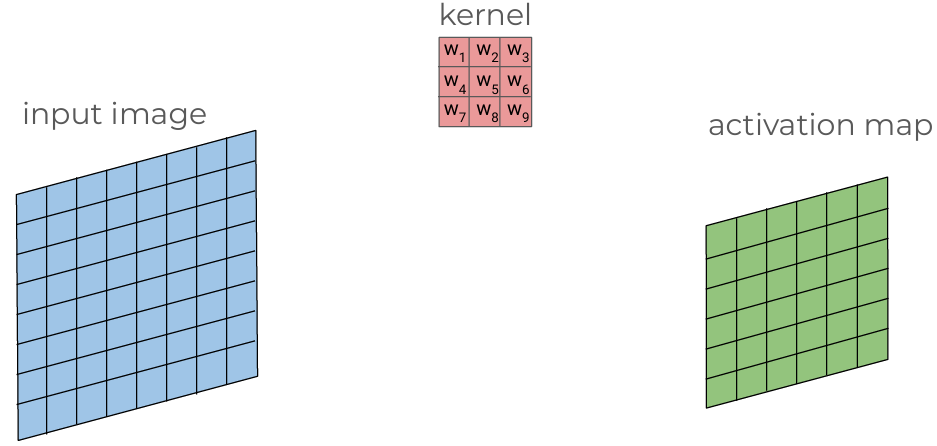
\includegraphics[width=0.8\linewidth]{figuresML/lesson_ml_3_pag_17.png}\hfill
        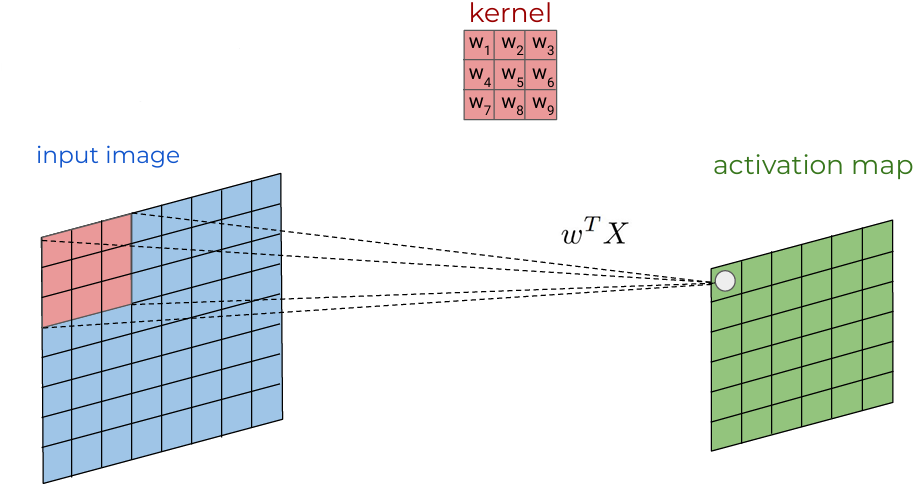
\includegraphics[width=0.8\linewidth]{figuresML/lesson_ml_3_pag_18.png} \\[.25cm] 
        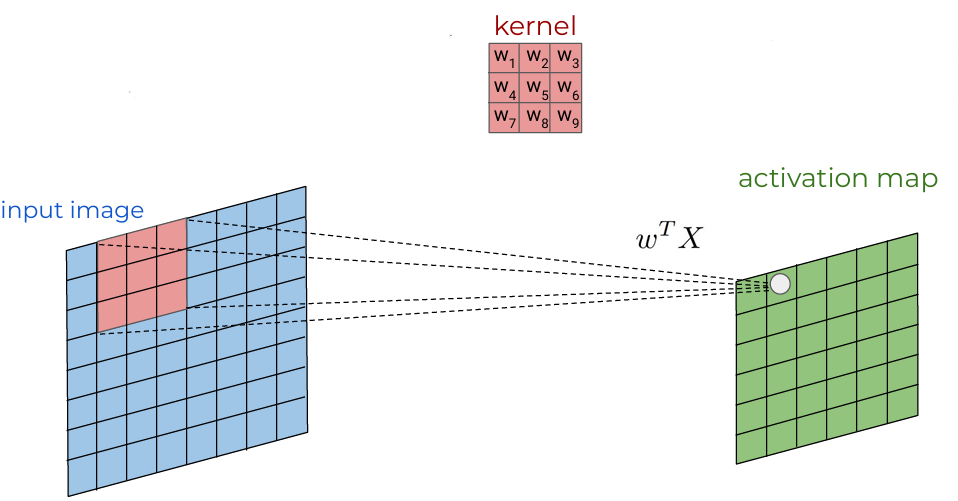
\includegraphics[width=0.8\linewidth]{figuresML/lesson_ml_3_pag_19.png}\hfill
        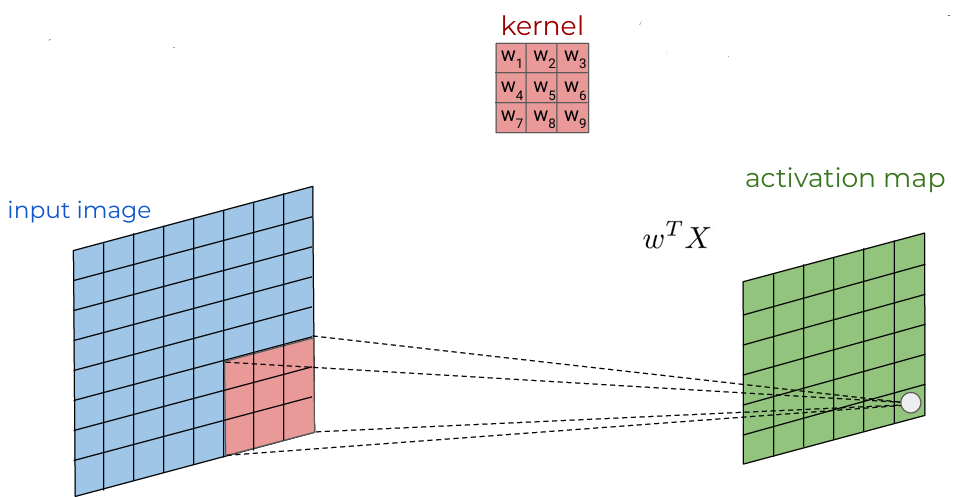
\includegraphics[width=0.8\linewidth]{figuresML/lesson_ml_3_pag_20.png}
    \end{minipage}
\end{figure} 
The idea of using a limited receptive field and of not connecting all the input pixels to all the neurons in the first layer comes from some biological hypothesis. In 1967, Hubel and Wiesel studied the response of the striate cortex in monkeys. They found that any small part of the striate cortex can be activated or suppressed in response to specific visual stimuli. So, animal vision is not performed by analysing each seen “pixel” but it works analyzing small part of the visual field. This led Fukushima in 1979 to invent the neocognitron, the first artificial neuron for vision.\\
We always use more than one kernel per layer (usually 32, 64, 128 and so on), and so we will have as many activation maps to work with. The figure below represents a typical convolutional layer, where each filter is learning a feature of the input image useful to solve our problem.
\begin{center}
    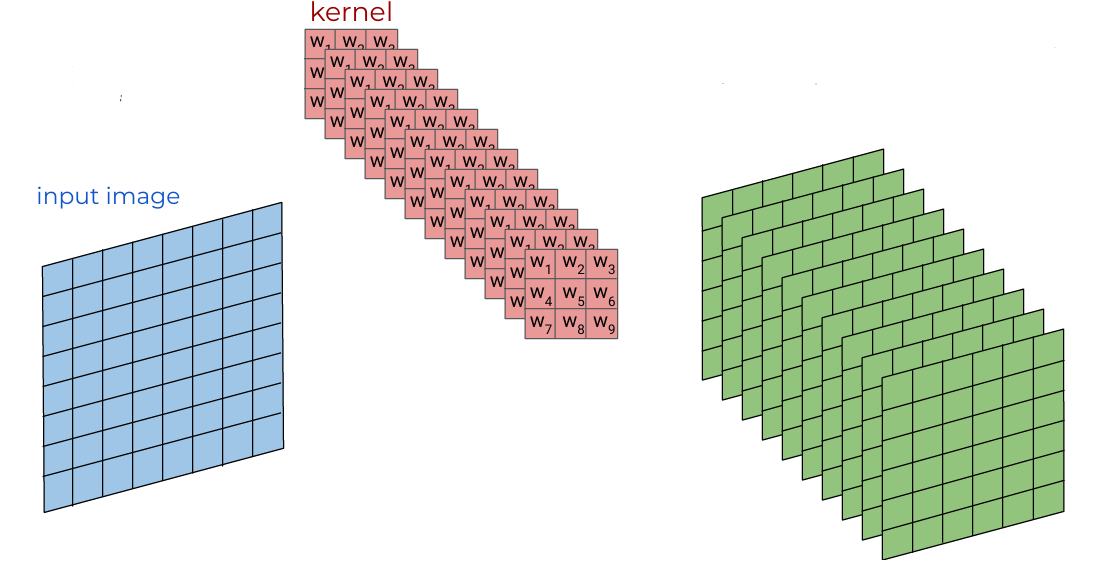
\includegraphics[width=0.6\linewidth]{figuresML/lesson_ml_3_pag_24.png}
\end{center}
Before the introduction of CNNs, the standard for computer vision was the so called \textit{feature engineering}, which is a method based on \textit{Sobel edge detection operators}. In practice these operators were kind of similar to filters, but their form was analytically defined a priori: finding filters, and hence features, capable of representing the information necessary to solve a complex problem (e.g classification of benign / malignant lesion in medical images etc...) was extremely complicated  and not as effective.

As you can see here, through the learning process, a CNN changes the value of the elements in the kernels to find the best representation of the data: it usually starts from simple features and then slowly learns the more complex ones (e.g. edges $\rightarrow$ textures $\rightarrow$ complex objects). It should be clear now that the \textbf{kernels themselves are the neurons of a CNN}, as they contain the trainable parameters.
\begin{center}
    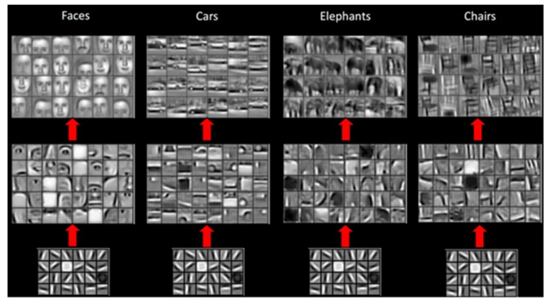
\includegraphics[width=0.6\linewidth]{figuresML/lesson_ml_3_pag_26.png}
\end{center}

Now that we understand the basics of CNNs we can ask ourselves \textit{why are CNNs so effective?} We can identify 3 main principles that make them so useful in the ML world:
\begin{enumerate}
    \item \textbf{Sparse connectivity:} Kernels slide over the image, meaning they connect only to a small, localized part of the input.
    \item \textbf{Sharing of parameters:} Through convolution, instead of learning a different set of parameters for each spatial position, the network learns only one set of weights per kernel. This induces... 
    \item \textbf{Translation invariance:} A feature is recognized regardless of its position in the image. For example, if a kernel is trained to recognize vertical lines, it doesn't matter where in the image the vertical lines is: thanks to parameter sharing and translation invariance it can be found wherever.
\end{enumerate}
Also, take a look at the following comparison: the number of parameters of a CNN is usually much smaller than the number of parameters of a classical NN with the same number of neurons.
\begin{center}
    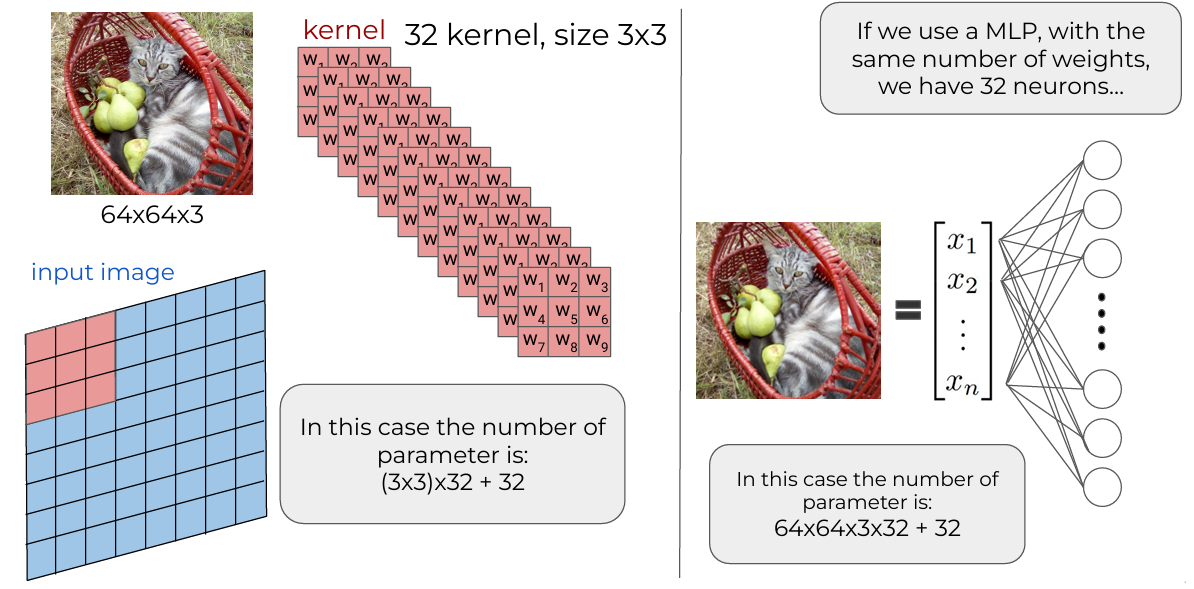
\includegraphics[width=0.75\linewidth]{figuresML/lesson_ml_3_pag_28.png}
\end{center}
\subsection{Structure of a Convolutional Neural Network}
As represented below, the typical structure of a CNN goes as follows:
\begin{itemize}
    \item[-] The input image is passed through:
    \begin{enumerate}
        \item A convolution operation;
        \item An activation function; 
        \item A pooling operation, which serves the purpose of compressing the information, drastically reducing the size of the activation maps (more information below).
    \end{enumerate}
    \item[-] All the operations are repeat layer after layer. 
    \item[-] The dimension of our data set is reduced step by step until we can flatten it and use a classifier algorithm like a NN.
\end{itemize}
\begin{center}
    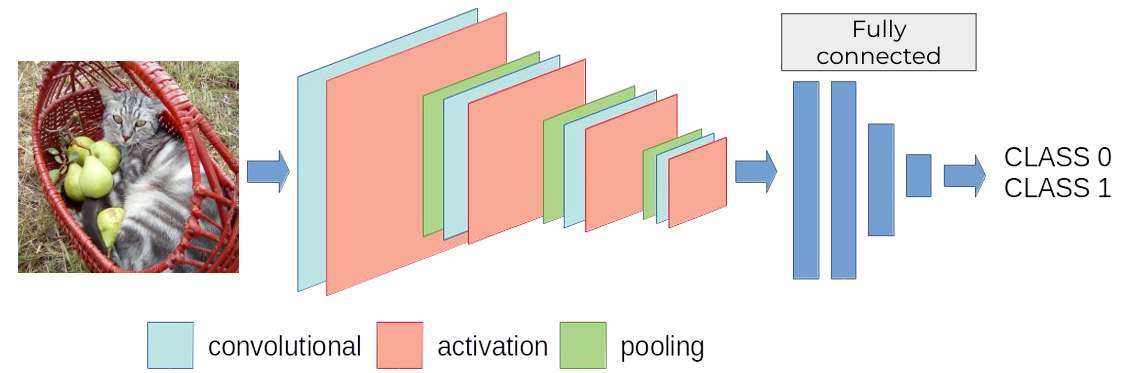
\includegraphics[width=0.8\linewidth]{figuresML/lesson_ml_3_pag_29.png}
\end{center}
Let's delve more deeply in the pooling process. \textbf{Pooling} is an invariant for permutation operation (such as a maximum or average) which is used, as said, to reduce the image / activation map size. As demonstrated below, applying a $2 \times 2$ max pooling operation with a stride of 2 involves extracting the maximum value from each non-overlapping $2 \times 2$ region of the input. The pooling window then shifts by two pixels (the stride) to evaluate the next block. Through this process, an initial $4 \times 4$ input tensor (or activation map) is downsampled into a compact $2 \times 2$ output tensor, effectively shrinking the size of the data while retaining the most prominent features.
\begin{center}
    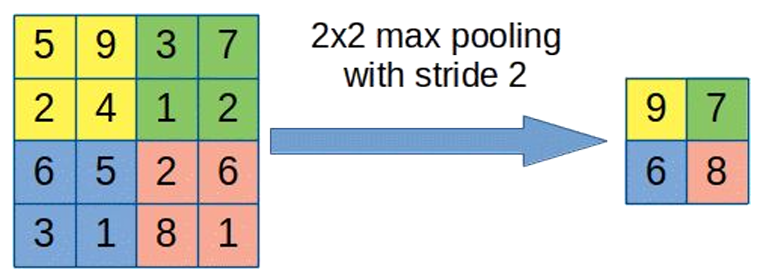
\includegraphics[width=0.35\linewidth]{figuresML/lesson_ml_3_pag_30.png}
\end{center}
Besides pooling, another method to reduce the size of the activation map and compress information is by increasing the stride of the convolution. As we have seen, the size of an activation map depends on the convolution parameters according to the formula:
\begin{equation*}
    M = \frac{N-k}{S} + 1
\end{equation*}
where $N$ is the image size (assuming an $N \times N$ image), $k$ is the filter/kernel size, and $S$ is the stride. What happens if we increase the stride? The resulting activation map becomes smaller. This introduces an alternative way to compress information, which raises an important question: is there a difference between using pooling and strided convolutions?

The key difference is that pooling does not add any parameters to the network; it is a fixed operation, meaning the network is not learning anything during this step and pooling just increases its efficiency. Conversely, a strided convolution relies on filters that contain trainable weights. In this case, we hope that the filters are not only learning to extract the necessary features to solve our task but are also simultaneously learning how to optimally compress the information. We cannot strictly control this behavior, as we simply rely on the optimization of the loss function. This highlights one of the main difficulties in developing neural networks: making numerous architectural choices (like whether to use a stride of 2, 3, or pooling instead) that can drastically change the model's performance.

Furthermore, we can "force" the convolution to slide over the entire image, including its edges, by using \textbf{padding}. Sometimes, we might want the output activation map to maintain the exact same spatial dimensions as the input (for instance, mapping a $64 \times 64$ input to a $64 \times 64$ output). Padding achieves this by adding extra pixels around the original image, allowing the kernel to start its convolution precisely on the boundaries, as shown below. The most common approach is zero-padding, but this can introduce strange artificial effects on the edges. Alternatively, one could pad using the average value of the overall image or the values of the corners. If the information at the edges of the image is crucial for the task, padding must be implemented carefully. Ultimately, this means there are many hyperparameters and design choices that must be fixed even within a single convolutional layer.

\begin{center}
    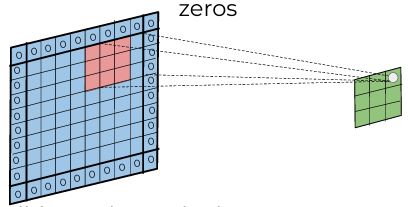
\includegraphics[width=0.35\linewidth]{figuresML/lesson_ml_3_pag_33.png}
\end{center}

We also mentioned that towards the end the input tensors can be flattened and fed into a classifier like a NN. We can do so in many ways, but the easier one would be to flatten the last activation $n \times m$ activation maps. The input of our classifier would then be a vector with length equal to  $n \times m \times a$ where  $a$ is the number of activation maps. This number can be too large with respect to the weights of the entire 
network. For example, if the last convolutional layer has 128 activation maps ($\rightarrow$ 128 kernels) with size $16 \times 16$ and the classifier is a fully connected NN with 100 neurons in the first layer, the number of parameters that are induced is $128 \times 16 \times 16 \times 100 = 3.276.800$. This problem is nearly always relevant due to the fact that \textit{it is convenient to choose a large number of small kernels in order to describe complex features} (we will say some more about this concept in a while). 

Instead, we could use \textbf{aggregation functions} in order to combine the data in the activation functions. The most common aggregation function is the \textbf{Global Average Pooling} (GAP), which consists in simply computing the average of each activation map (so each one is collapsed into a single number) and then vectorizing the result. In the previous example, the number of parameters is reduced to $128 \times 100 = 12.800$ (number of activation maps times number of neurons in the first layer of the NN).

Finally, if the last classifier is a NN, \textit{we can train the entire structure end-to-end}, as seen in previous chapters, by defining a loss function, applying backpropagation, and optimizing the parameters. This has some advantages, like a better accuracy for kernel parameters. However, we can also use the CNN strictly as a \textbf{feature extractor}, i.e. an instrument that translates a complex input image in a simple numerical vector. In this case, the output from the flattening, can be used directly as input features to feed a completely different machine learning algorithm, such as a Decision Tree. We will explore this approach later when discussing Transfer Learning.

\subsection{Evolution of CNN Architectures}

The easiest way to improve a CNN algorithm is finding a way to extract and comprehend more precisely and efficiently, for example by building deeper and deeper networks. However, this requires hardware able to withstand an enormous amount of computation: not every problem can be solved by a bigger GPU, and one of the most important factors of progress in the ML world is also finding ways to reduce the computational cost of training. These are the two main research goals in the field.

With said, let's briefly review the recent history and improvements of CNNs by looking at some of the most important examples of CNNs:

\begin{center}
    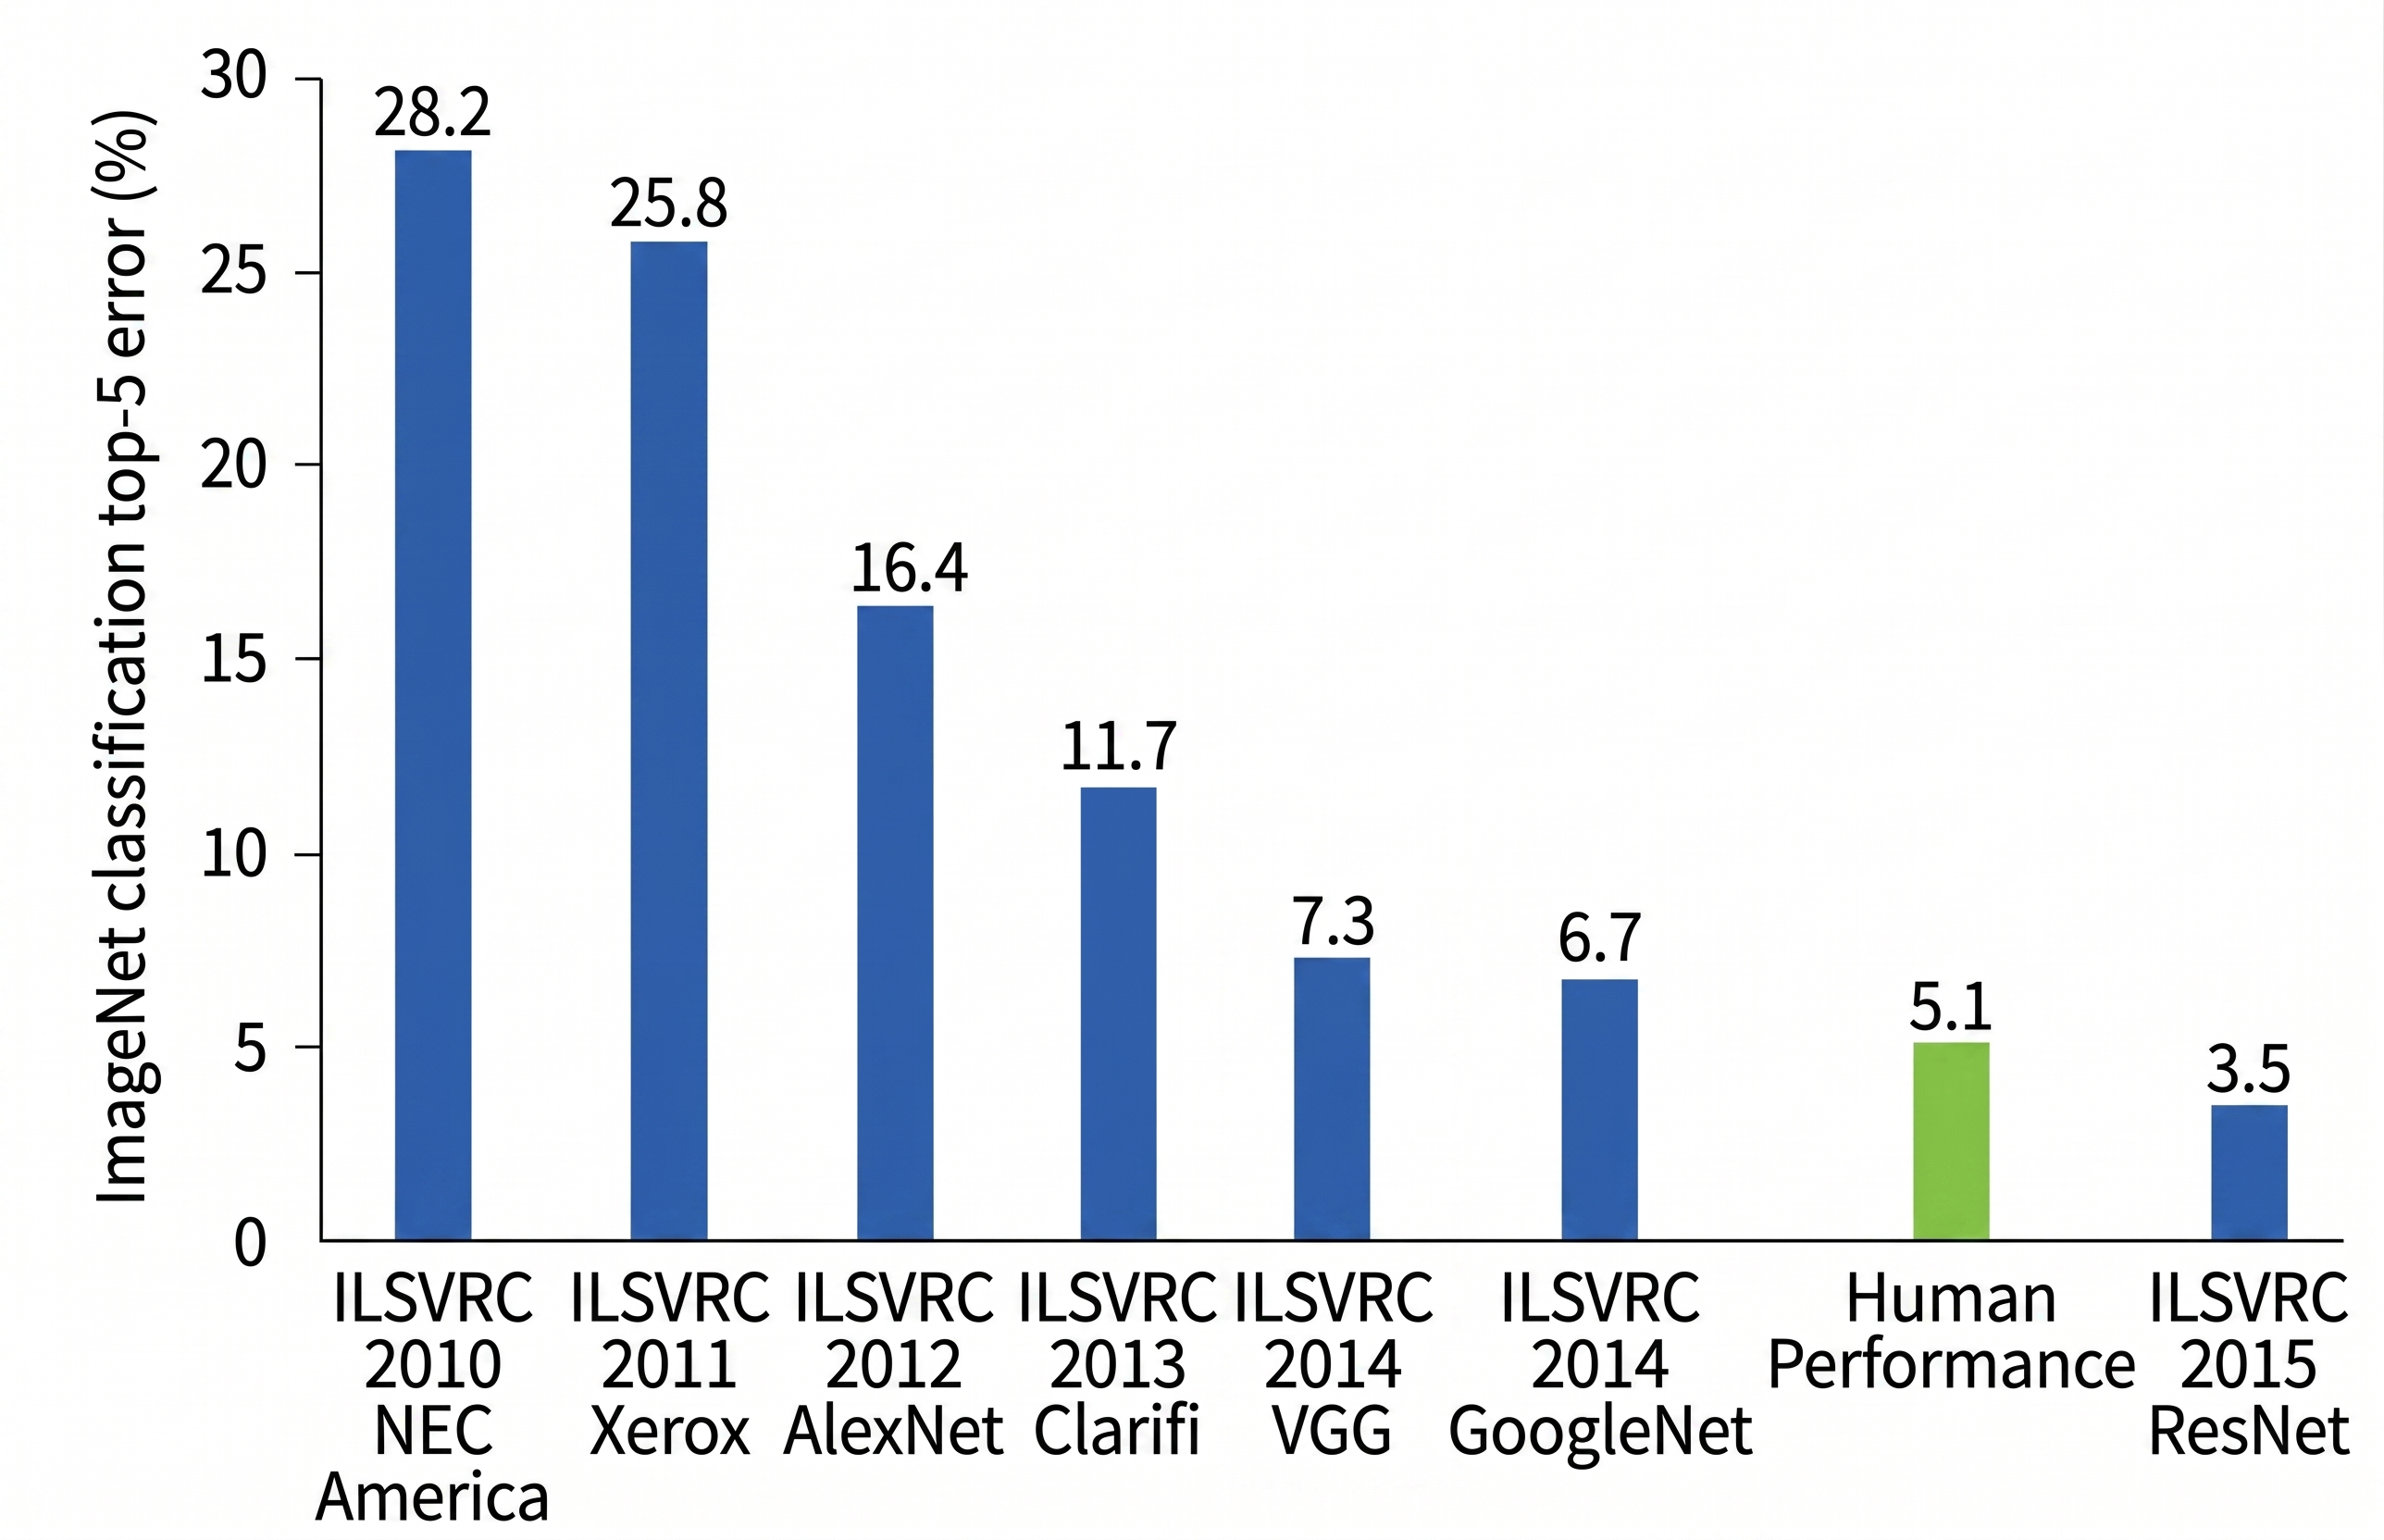
\includegraphics[width=0.45\linewidth]{figuresML/lesson_ml_3_pag_46.png}
\end{center}

\textbf{- AlexNet (2012):} Created by Alex Krizhevsky et al., AlexNet had 8 convolutional layers and outperformed all competitors in the ILAVRC by combining a series of previous revolutionary work with important innovations like:
\begin{itemize}
    \item[-] The neocognitron, proposed by Kunihiko Fukushima in 1979;
    \item[-] A backpropagation algorithm, a term coined by Rosenblatt in 1962 and which evolved greatly between the 1970s and the early 2000s;
    \item[-] LeNet, proposed by Yan LeCunn in 1998;
    \item[-] GPU acceleration first proposed by Kumar Chellapilla;
    \item[-] A new (for the time) activation function: the ReLU;
    \item[-] Data augmentation and many other "small" adjustments;
\end{itemize}

\textbf{VGG19 (2014):} In 2014, a network called VGG19 with 19 layers by Karen Simonyan and Andrew Zisserman won the ImageNet competition. The main difference that led them to improve the design of AlexNet by being able to add more layers is a clever implementation of the pooling system. AlexNet: contemplates the use of convolution filters of different sizes, from largest to smallest: $11 \times 11$, $5 \times 5$, $3 \times 3$ and then $3 \times 3$ throughout the architecture. With this structure, the number of parameters for the $11 \times 11$ layer is $11 \times 11 \times 32 = 3872$ where 32 is the number of filters. Istead of using “large” filters ($11 \times 11$ or $5 \times 5$), VGG19 uses small ones sequentially before pooling. Five $3 \times 3$ filters in sequence have an \textbf{effective receptive field} of $11 \times 11$ with a smaller number of parameters: $3 \times 3 \times 32 \times 5 = 1440$ where 32 is the number of filters and 5 the number of layers. It is therefore possible to go deeper by reducing the number of learnable (trainable) parameters. 

What exactly do we mean with effective receptive field? The effective receptive field is the spatial extent of the original input image that contributes to the calculation of a single pixel in a given activation map. As illustrated in the comparison below, a single $5 \times 5$ convolution directly looks at a $5 \times 5$ area of the input. However, if we stack two $3 \times 3$ convolutional layers, the first layer processes $3 \times 3$ regions, and the second layer processes $3 \times 3$ regions of those intermediate activations. Ultimately, a single pixel in the output of the second layer implicitly depends on a $5 \times 5$ region of the original input. 

Both approaches "look" for correlations at the exact same points in the input image, maintaining an effective receptive field of $5 \times 5$. The critical advantage lies in parameter efficiency: assuming 32 channels, a single $5 \times 5$ layer requires $5 \times 5 \times 32 = 800$ parameters. In contrast, the two stacked $3 \times 3$ filters require only $3 \times 3 \times 32 \times 2 = 576$ parameters. This principle allowed VGG19 to stack many more layers, increasing the non-linearity and depth of the network while keeping the computational cost manageable.

\begin{center}
    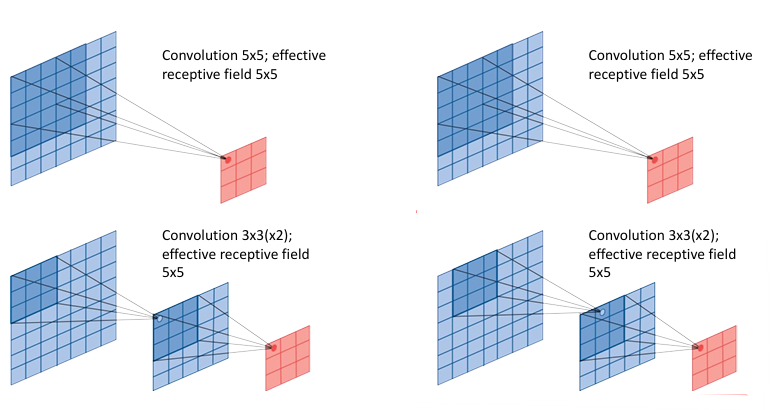
\includegraphics[width=0.7\linewidth]{figuresML/lesson_ml_3_pag_49.png}
\end{center}

\textbf{InceptionLeNet (2014):} In 2014 the InceptionNet 22 layers CNN won the ImageNet competition. It implemented an architecture that was used to search for representations at multiple scales: the input (or simply the output of the previews layer) was passed through multiple \textit{parallel} layers with filters of different sizes and then the filters output was concatenated with various techniques, as represented here.

\begin{center}
    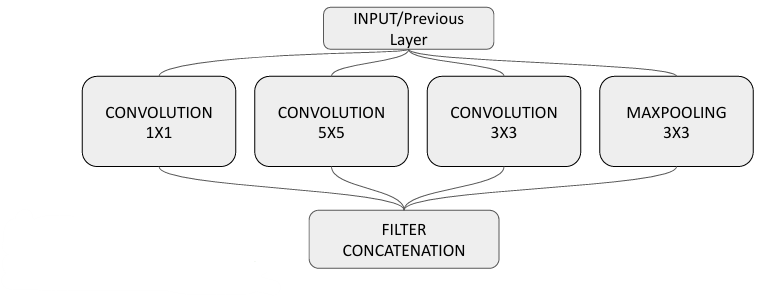
\includegraphics[width=0.6\textwidth]{figuresML/lesson_ml_3_pag_54.png}
\end{center}

This method, however, has a serious problem: the number of parameters explodes. In this naive configuration, applying multiple parallel filters (such as $1 \times 1$, $3 \times 3$, and $5 \times 5$ convolutions) directly to an input with a high number of channels results in a massive computational cost. For example, even with a relatively small input depth and a limited number of filters per convolution, the parameter count quickly skyrockets. To solve this, the so called \textbf{inception block} introduces a clever workaround: it adds $1 \times 1$ convolutions before the more expensive $3 \times 3$ and $5 \times 5$ convolutions, as well as after the max pooling layer. These $1 \times 1$ convolutions serve to reduce the depth of the input data (i.e., the number of channels from the previous block). 
For example, consider an input with 256 channels and a target of 32 output filters using a $5 \times 5$ convolution:
\begin{itemize}
    \item \textit{Naive approach:} A direct $5 \times 5$ convolution requires $5 \times 5 \times 256 \times 32 = 204,800$ parameters.
    \item \textit{Inception approach:} Using a $1 \times 1$ convolution to first reduce the input depth (as shown below) to 16 channels requires $(1 \times 1 \times 256 \times 16) + (5 \times 5 \times 16 \times 32) = 4,096 + 12,800 = 16,896$ parameters. 
\end{itemize}
This simple bottleneck step eliminates over 90\% of the computational cost. By shrinking the dimensional depth before applying larger kernels, InceptionNet drastically reduces the total number of trainable parameters, making the architecture computationally viable while still successfully capturing multi-scale representations.

\begin{center}
    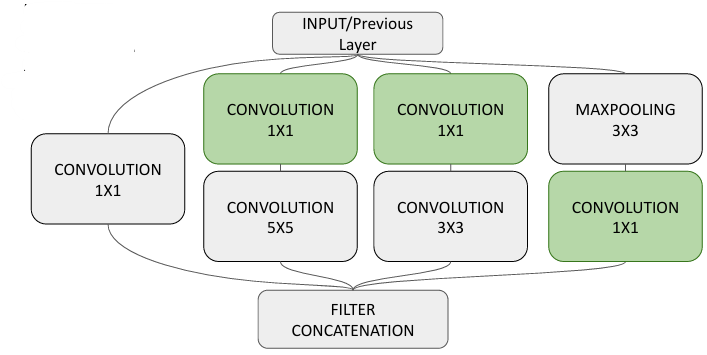
\includegraphics[width=0.5\textwidth]{figuresML/lesson_ml_3_pag_57.png}
\end{center}

\begin{figure}[H]
    \begin{minipage}[c]{0.54\textwidth}
    Here is a figure taken from the original InceptionNet paper. As you can see the input data is processed through the other convolutional layers before entering the inception block. This ensures that the size of the data at the input of the inception block is $a \times b \times F$ where $F$ of filters of the previous layer and $a \times b$ is the size of the previous activation function. \newline \newline
    \textbf{ResNet(2015)}: A massive jump in depth was achieved by the ResNet CNN, which featured 152 layers and exceeded the human capabilities in the classification task of the ImageNet competition. As we already mentioned hundreds of times, as the number of layers increases, the number of neurons increases and so does the number of trainable parameters. Note that when the computational cost becomes higher and higher, not only you are going to need for higher performance GPUs (in particular VRAM), but you will also face simple logistics problem during development: if the algorithm you want to train takes 2 weeks to run, it will be more complicated to develop since you will be able to debug it only twice a month!
    \end{minipage}\hfill 
    \begin{minipage}[c]{0.45\textwidth}
        \centering
        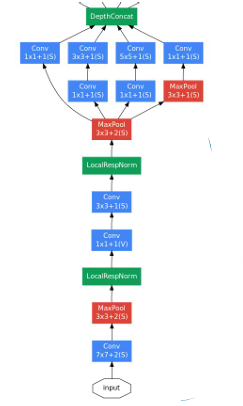
\includegraphics[width=0.8\linewidth]{figuresML/lesson_ml_3_pag_58.png}\hfill
    \end{minipage}
\end{figure} 

\subsection{The vanishing gradient problem}\label{sec:skip_connections}

There is another problem specific to CNNs (but also true for NN): the nightmare of the vanishing gradient. As said, training a CNN means using backpropagation to update the weights once the loss function has been calculated and it requires the calculation of many derivatives. Close to convergence, when the neural network is close to a local minimum of the cost function, the variations in the weights will become very small, which means the derivatives of the loss with respect to this small changes will be very small, close to 0. Applying the chain rule for calculating the gradient simply means that, to update the weights of the neural network, we must multiply many of these derivatives. Multiplying many small factors leads to gradients approaching zero and that is the so called \textbf{vanishing gradient problem}. 

Such problem has many causes, for example a wrongful choice for the activation function. If you look at a sigmoid, it is easy to see that as $x$ increases, the derivative of the function goes to zero, which does not happen for the ReLu. However, the fact that for negative values the ReLu is zero can cause some problems, easily manageable by changing the activation function to a Leaky ReLu or some other variant. 

Wrongful weight initialization can also cause the same problem. Consider the following example.
\begin{center}
    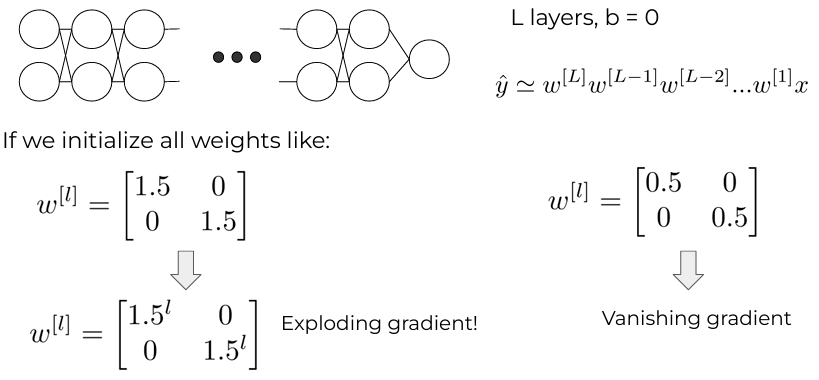
\includegraphics[width=0.6\textwidth]{figuresML/lesson_ml_3_pag_71.png}
\end{center}
Given the $L$ layers of the DNN, if we initialize all weights with values smaller than 1 (for example, $0.5$), repeated multiplications across the layers during backpropagation will result in terms proportional to $0.5^L$. For deep networks, this value quickly approaches zero, causing the vanishing gradient. Conversely, initializing weights with values strictly greater than 1 (like $1.5$) will result in terms proportional to $1.5^L$, which rapidly grow out of control and lead to an exploding gradient.

There are many ways to correctly initialize weights that have been proven to work in an empirical way. Given the complexities of DL algorithms, it should not come as a surprise that sometimes we just need to rely on practice to make something work even if we cannot comprehend \textit{why} it works a priori. Here are some examples:
\begin{itemize}
    \item[-] \textit{Random initialization}: sampling the weights from a normal distribution or a uniform distribution, usually independently.
    \item[-] \textit{LeCun initialization}: it is designed to preserve the variance of neural activations during the forward pass. It samples each entry $W(l)$ independently from a distribution with mean 0 and variance $1/n_{l-1}$.
    \item[-] \textit{Glorot initialization}: it preserves activation variance during the forward pass and gradient variance during the backward pass.
    \item[-] \textit{He initialization}: Since Glorot initialization performs poorly with ReLU, we can use
    \begin{equation*}
        w^{[l]}=\sqrt{\frac{2}{n^l + n^{(l-1)}}}
    \end{equation*}
\end{itemize}

Lack of \textit{batch normalization} can also lead to a vanishing gradient.It consists in the normalization of the inputs of each layer so that they have a stable distribution during training. It is typically applied after the convolutional layer and before the activation function (like ReLU), calculating $\hat{x} = \frac{x - \mu}{\sqrt{\sigma^2 + \epsilon}}$ computed on a batch of data. It was introduced to address the problem of \textbf{internal covariate shift}:
\begin{itemize}
    \item[-] When weights in earlier layers change, the outputs of those layers also change.
    \item[-] These outputs become the inputs for the next layer, so their statistical properties (mean, variance) shift.
    \item[-] This forces subsequent layers to constantly adapt to new input distributions, making training harder.
\end{itemize}
Without this normalization step, the network suffers from slower training, requires smaller learning rates, and becomes highly susceptible to exploding or vanishing gradients.

Lastly, we said that as we try to build deeper networks, the number of multiplications required to compute derivatives during backpropagation increases significantly and if these individual derivatives are close to zero, multiplying many of them together inevitably leads to the vanishing gradient problem. To solve this, we must find a way to decrease the number of multiplications required for the gradient. The solution comes in the form of \textbf{residual skip connections}, which are connections bridging non-adjacent layers, as shown in figure. This mechanism is the foundational idea behind the ResNet architecture.

\begin{center}
    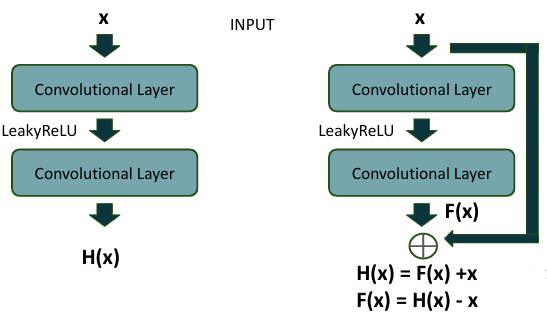
\includegraphics[width=0.5\textwidth]{figuresML/lesson_ml_3_pag_78.png}
\end{center}

Instead of forcing the network to learn a direct mapping entirely through stacked convolutional layers, skip connections introduce an identity mapping. If the output of a block of convolutional layers is $F(x)$ and the original input to that block is $x$, the skip connection directly adds the input to the output. This results in the final mapping is $H(x) = F(x) + x$. \\ 
This simple addition has a profound mathematical impact during backpropagation: when computing the gradient with respect to $x$, the derivative becomes $\frac{\partial F}{\partial x} + 1$. The addition of the $+1$ ensures that even if $\frac{\partial F}{\partial x}$ becomes infinitesimally small, the overall gradient will not vanish. 
Implementing skip connections provides several key advantages:
\begin{itemize}
    \item[-] Enables deeper networks.
    \item[-] Mitigates the vanishing gradient.
    \item[-] Improves convergence speed (the network learns faster because the gradient has shorter, direct paths to earlier layers).
    \item[-] Preserves fine details (original input information bypasses intermediate transformations, maintaining fine-grained details better throughout the network).
\end{itemize}

\subsection{Notes on explainability and transfer learning}

CNNs dramatically changed the trajectory of Neural Networks and AI. Their success in computer vision proved that deep architectures could outperform traditional methods, which fueled massive interest and investment in deep learning. This breakthrough laid the foundation for subsequent advances, including architectures like transformers that power models such as GPT. After the 2017 edition, the ImageNet competition was officially closed and today it remains one of the totems of the massive progress the field experience during the 2010s. Today Convolutional Neural Networks are still very powerful models but as any other deep learning algorithm they can be considered black boxes: this simply means that we cannot fully understand why they take certain decisions as we may have million of million of trainable parameters. There is an entire branch of AI research called eXplainable AI (XAI) that aim to develop method to explain NN. One of the most used method for CNN is called \textit{gradCAM} which exploits the global average pooling (we will not be focusing on this, you can research it on your own if interested).

Another fundamental concept in modern Deep Learning is \textbf{transfer learning}. In many real-world scenarios, we might want to leverage the power of a complex CNN, but we simply do not have enough data to train such a massive algorithm from scratch. To overcome this limitation, we can exploit the structural composition of a CNN, which (as we saw before) is essentially divided into two main components: the \textbf{convolutional part} (which acts as a \textit{feature extractor}) and the \textbf{classifier} (typically a fully connected NN or MLP). By training the entire network on a very large, generalized dataset first, we can reuse it for our specific, smaller dataset using two main strategies:
\begin{itemize}
    \item[-] \textbf{Feature Extraction:} We split the network and use only the first part. The pre-trained convolutional layers extract the features from our new data, and this output (after a flattening or global average pooling step) is then used as the input for a new, independent classifier. \\ Example: Using a CNN pre-trained on ImageNet (millions of general images) to extract basic shapes and textures, and training only a new, simple classifier on top to recognize specific flower species.
    \item[-] \textbf{Fine Tuning:} We take the pre-trained network, change a small portion of the architecture, and train the whole system again to fit our specific data. Common modifications include adapting the input (e.g., adjusting to smaller/bigger images, or switching between grayscale and RGB) or modifying the output (e.g., replacing the final layer of a network originally trained for 100 classes so that it can perform a simple binary classification). \\ Example: Taking an ImageNet model, replacing its 1000-class output layer with a 2-class layer, and gently re-training the entire network to adapt its filters for detecting tumors in medical X-rays.
\end{itemize}
